\documentclass[17pt,landscape]{extarticle} 

%\usepackage[margin=0.5in]{geometry}
\usepackage[left=0.5in,right=0.5in,top=0.5in,bottom=0.5in]{geometry}

\usepackage{graphicx}

\usepackage{amsmath,amssymb}

\usepackage{url,hyperref}



\newcommand{\mywidth}{0.3\textwidth}

\newcommand{\comment}[1]{}


\title{Computational Medicine\\Computational Anatomy\\Homework 3}
%\title{Homework 3}
\author{Computational Anatomy}
\date{}

\begin{document}
\maketitle

% no numbering
\thispagestyle{empty}
\pagestyle{empty}
%\setcounter{page}{27}



\comment{
\section{Euler Lagrange solution to a hanging mass spring system}

Consider a one dimensional system consisting of an object with mass $m$, hanging from a spring with constant $k$ under the influence of gravity with acceleration $g$ (a positive number).

Use the coordinate $\varphi$ to represent the displacement of the mass from the spring's equilibrium length and $\dot \varphi$ to represent its velocity.

\subsection{}
Write down the potential energy of the system.  This should include gravitational potential and spring potential.  Check the mass spring problem and the cannonball problem in the notes to understand these two potential energy terms.


Write down the kinetic energy of the system.


Write down the Lagrangian $L$ (kinetic energy minus potential energy).

\subsection{}
Calculate $\frac{\partial}{\partial\varphi} L$ ,  $\frac{\partial}{\partial\dot\varphi} L$ and $\frac{d}{dt}\frac{\partial}{\partial\dot\varphi} L$.

\subsection{}
Write down the differential equations of motion using the Euler Lagrange equation.  

\subsection{}
Solve the differential equations to give a general solution.  Note there should be two free parameters corresponding to initial conditions $\varphi_0,\dot\varphi_0$.   Hint: make a change of variables $\psi = \varphi + c$ for some constant $c$ to give a homogeneous differential equation in $\psi$, noting that $\dot \psi = \dot \varphi$.
}

\section{Image matching with translation}

We consider aligning a 2D template image $I$ to a 2D target image $I'$ using translation only.

We want to find the vector $b$ that minimizes the cost
\begin{align*}
C(b) = \frac12 \int |I(x - b)  - I'(x)|^2 dx
\end{align*}

\subsection{}
Consider the perturbation $b \mapsto b + \epsilon h$ and write
\begin{align*}
J(\epsilon) = C(b + \epsilon h)
\end{align*}
Work out
\begin{align*}
\left. \frac{d}{d\epsilon}  J(\epsilon ) \right|_{\epsilon = 0}
\end{align*}

\subsection{}
Write down the gradient of the cost with respect to $b$.  Recall that $\nabla C(b) \cdot h = \frac{d}{d\epsilon} J(\epsilon)\big|_{\epsilon = 0}$.  

\subsection{}

Write down a gradient descent algorithm that can be used to minimize this cost for a given $I$ and $I'$.  It should take the form of
\begin{align*}
b_{\text{new}} = b_{\text{old}} - \epsilon\left( \text{gradient term} \right)
\end{align*}
for $\epsilon$ a small step.

\subsection{}
Write a program in matlab that will implement this algorithm.  The inputs should be the template image $I$, the target image $I'$ (both 2D arrays), the gradient descent step size $\epsilon$, and the number of iterations of gradient descent.

The program should output the optimal vector $b$, and the transformed image $I(x - b)$.

Note that you can use matlab's built in function \verb$gradient$ to compute the gradient of the image.

One method you can use to apply the translation to $I$ is
\begin{verbatim}
[X,Y] = meshgrid(1:size(I,2),1:size(I,1));
I_translated_by_b = interp2(I,X-b(1),Y-b(2),'linear',0);
\end{verbatim}

You should print the cost $C$ at each iteration of gradient descent to make sure it is decreasing.  If it is not decreasing, choose a smaller step size.

You may use the given code \verb$splineImage.m$ as a model for your program.  You will notice a lot of similarities, but your program will be simpler.  For example, you will not need the function \verb$applyPowerOfA$.  You will not need the input arguments \verb$alpha$ or \verb$sigma$.  Remember that your gradient will be a vector with 2 components.  It will not be a function at each point in space like in \verb$splineImage.m$.

\subsection{}
Use your code to match the corpus callosum \verb$0001_CC_Con.png$ to \verb$0003_CC_Alz.png$ with translation.  You can view the whole MRI these structures are segmented from in the files \verb$0001_MRI_Con.png$ and \verb$0003_CC_Alz.png$ if you wish.

You can load them like this 
\begin{verbatim}
I = double(imread('0001_CC_Con.png') > 0);
IPrime = double(imread('0003_CC_Alz.png') > 0);
\end{verbatim}
This image should now take two values only, 0 and 1, and be represented in double precision, not with an 8 bit integer.  You can see what these images look like in Fig. \ref{fig:CC}

\begin{figure}
\centering
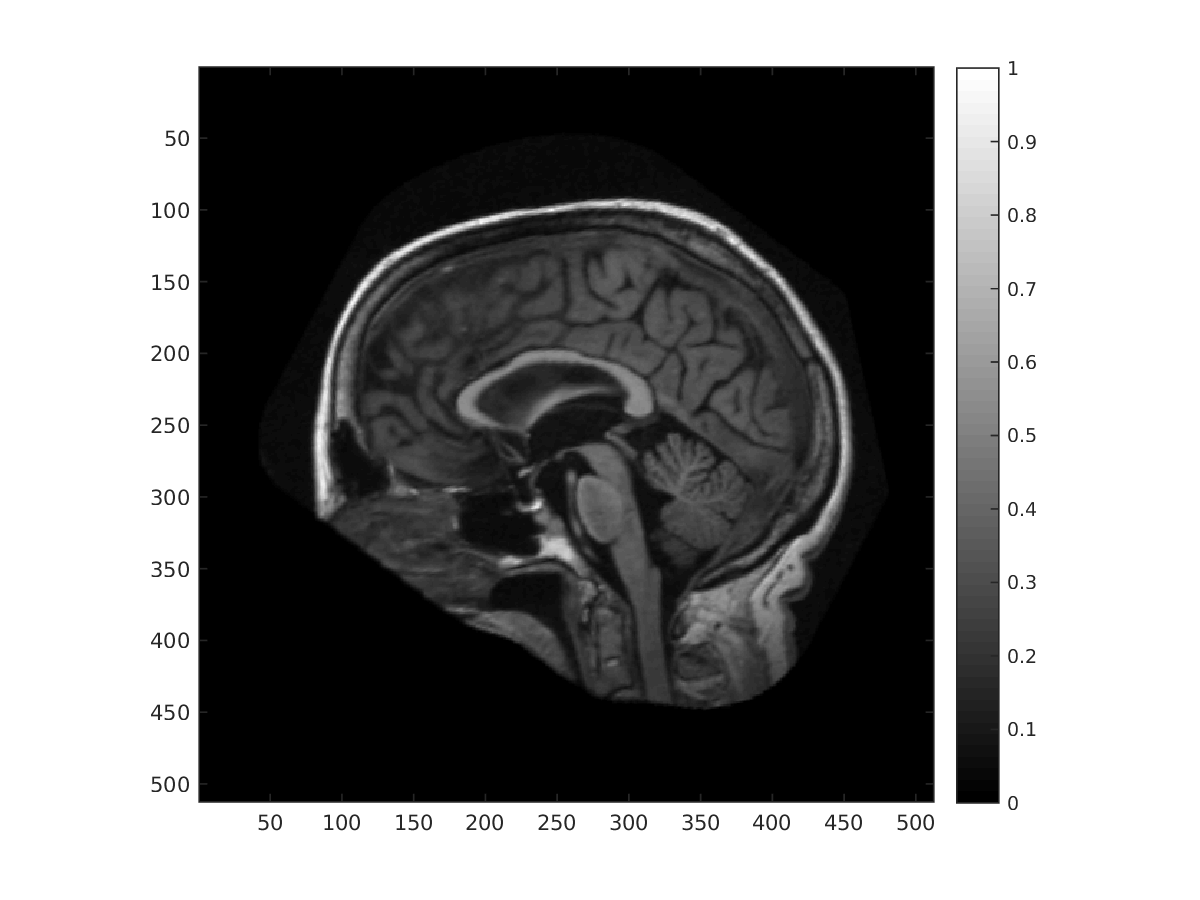
\includegraphics[width=0.4\textwidth]{MRI_Con.png}~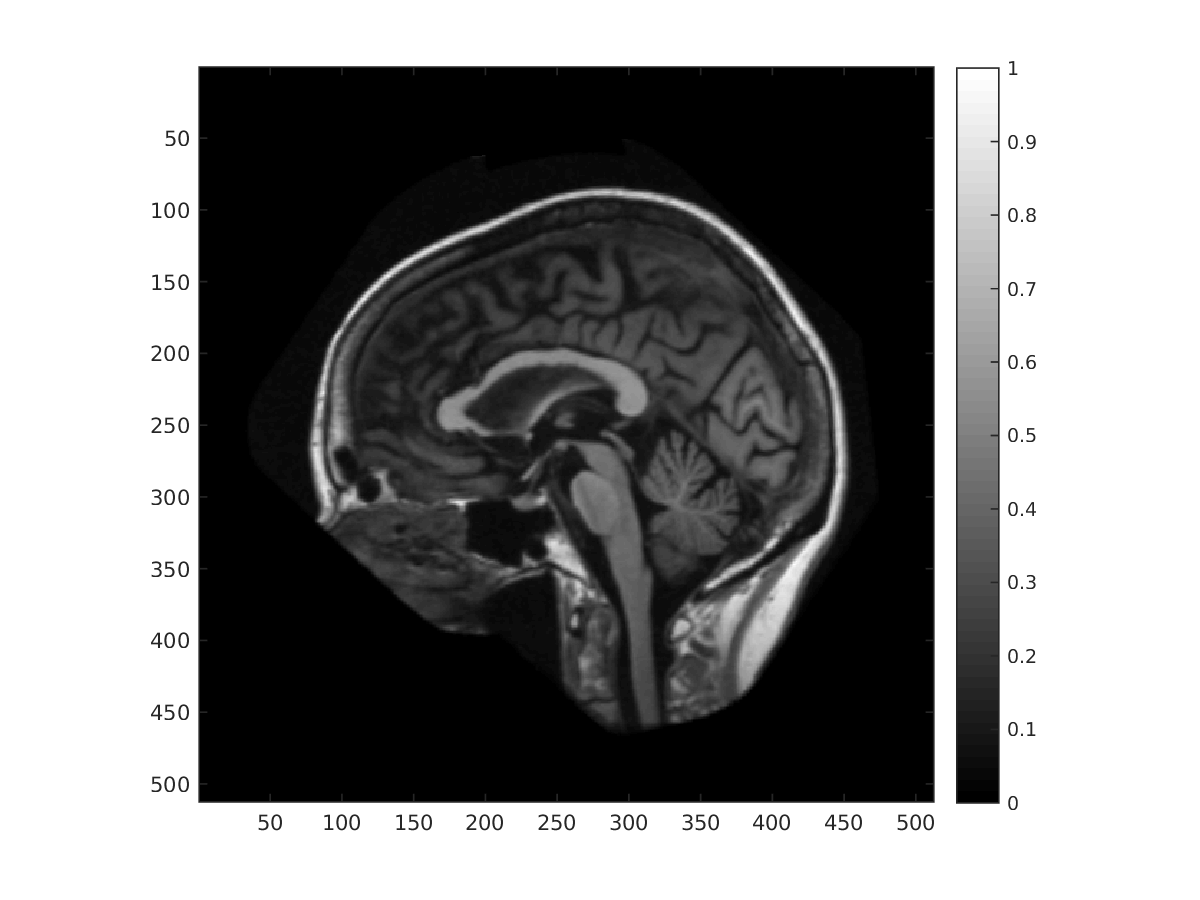
\includegraphics[width=0.4\textwidth]{MRI_Alz.png}
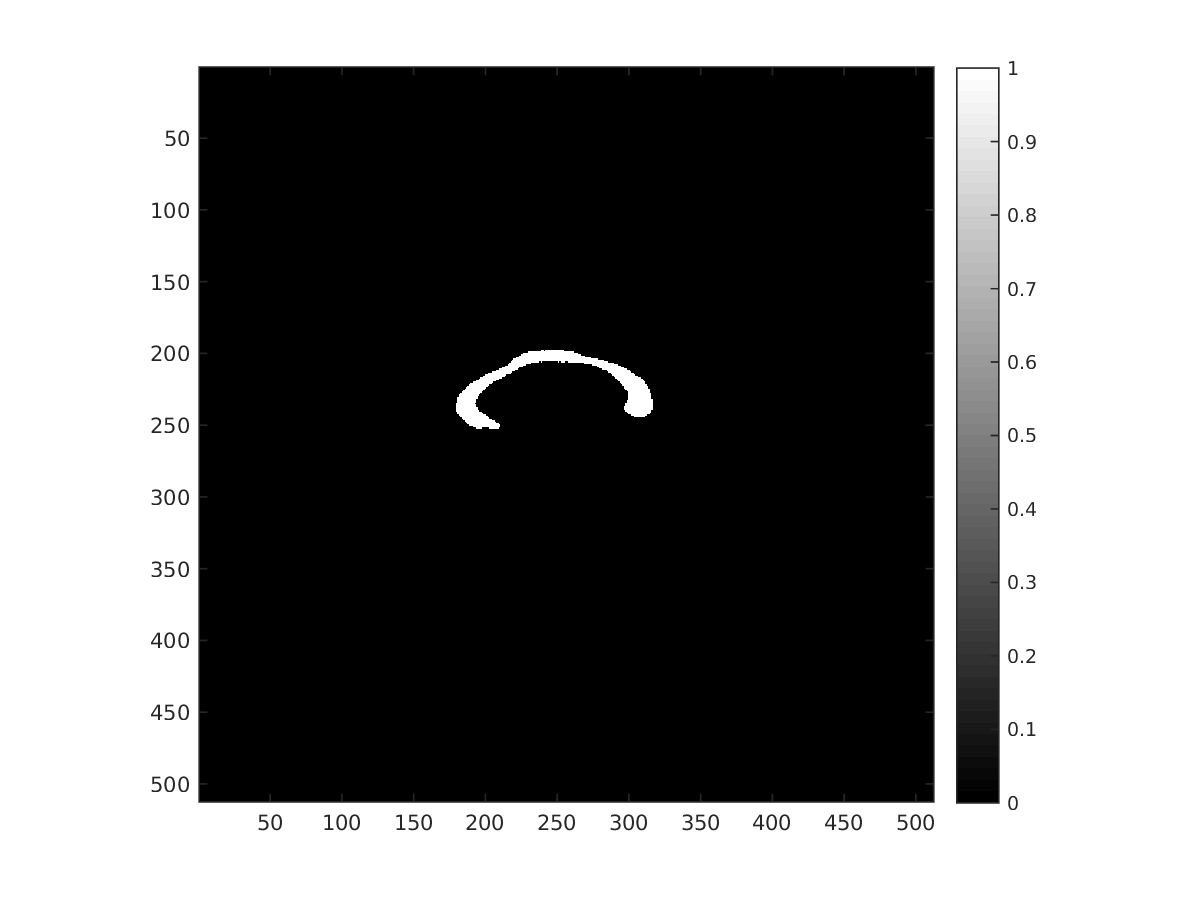
\includegraphics[width=0.4\textwidth]{CC_Con.png}~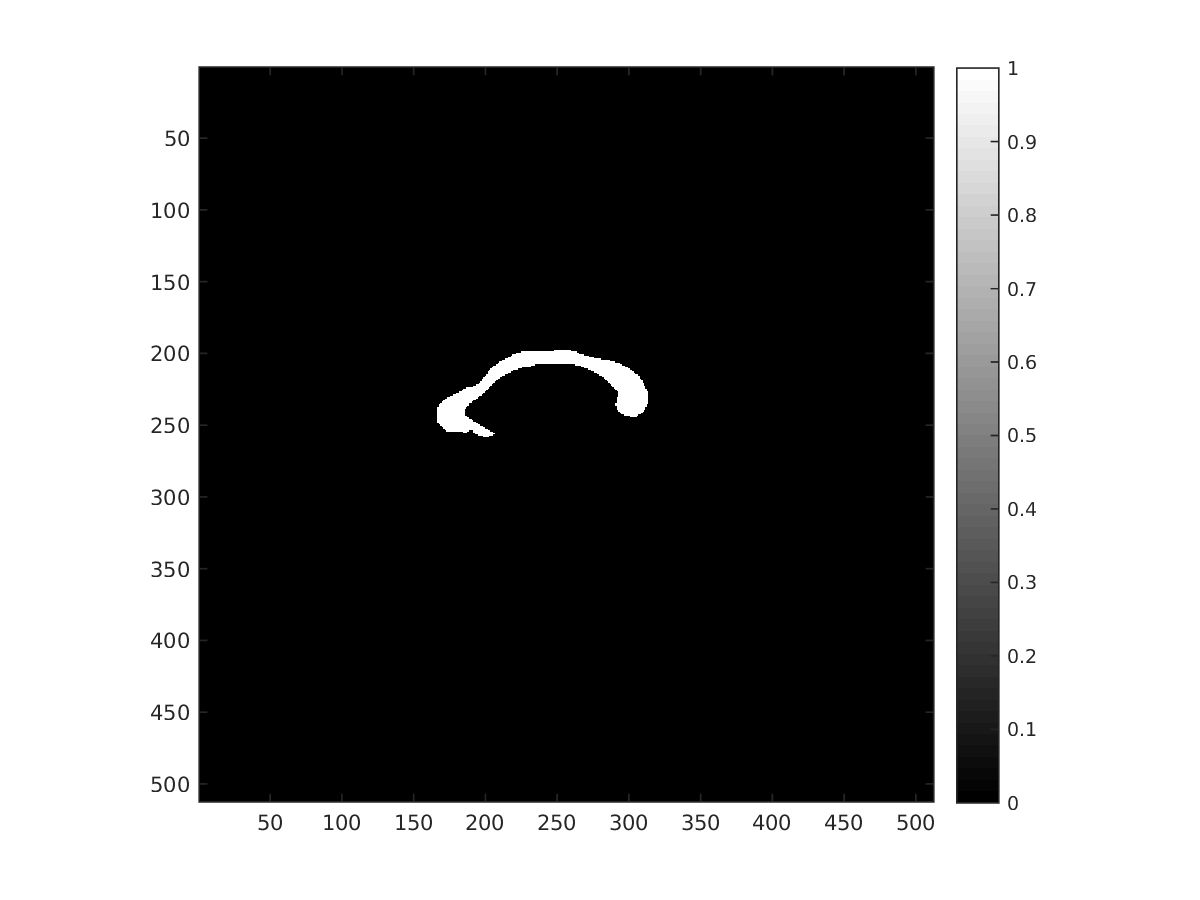
\includegraphics[width=0.4\textwidth]{CC_Alz.png}
\caption{\label{fig:CC} Corpus callosum for control (left) and Alzheimer's (right)  subjects used for this exercise, shown with colorbar.}
\end{figure}

Report the step size you used and the number of iterations.  Report the initial cost, and the final cost after your algorithm is finished.  Report the two values in the translation vector $b$.

Make a figure showing the template image, the translated template image, and the target image.

Make a figure showing the template image minus the target image, and the translated template image minus the target image. Include a colorbar.



\subsection{Image matching with splines and Jacobian calculations}

\subsection{}

Use the given code \verb$splineimage.m$ to match your translated corpus callosum to your target.  If you were unable to complete the previous part of the homework  then just use the original (untranslated) corpus callosum.

Use the value $\sigma = 0.01$.  This parameter controls how important matching accuracy is relative to the size of the deformation. 

Use the value $\alpha = 20$.  This parameter controls how smooth the deformation is.

Report the step size you used and the number of iterations.  Report the initial cost, and the final cost after your algorithm is finished.  Again, if the cost is not decreasing, choose a smaller gradient descent step size.

Make a figure showing the deformed image.  Make a figure showing the deformed image minus the target image. Include a colorbar.

\subsection{}
Calculate the determinant of Jacobian of the transformation $\varphi(x) = x + v(x)$ at each point in space.  Show this in a figure with a colorbar.






\end{document}
